\documentclass[11pt]{article}

\usepackage[utf8]{inputenc}
\usepackage[T1]{fontenc}
\usepackage{lmodern}
\usepackage[margin=0.92in]{geometry}
\usepackage{amsmath,amssymb,mathtools,bm}
\usepackage{booktabs,tabularx,array,multirow,longtable}
\usepackage{graphicx}
\usepackage{microtype}
\usepackage{xcolor}
\usepackage{enumitem}
\usepackage{siunitx}
\usepackage{float}
\usepackage{subcaption}
\usepackage{hyperref}
\usepackage{cleveref}
\usepackage{tikz}
\usepackage{pgfplots}
\usetikzlibrary{arrows.meta,positioning,fit,calc,matrix,backgrounds}
\pgfplotsset{compat=1.18}

\hypersetup{
  colorlinks=true,
  linkcolor=blue!45!black,
  citecolor=blue!45!black,
  urlcolor=blue!45!black
}

\newcommand{\E}{\mathbb{E}}
\newcommand{\Var}{\operatorname{Var}}
\newcommand{\Cov}{\operatorname{Cov}}
\newcommand{\diag}{\operatorname{diag}}
\newcommand{\R}{\mathbb{R}}
\newcommand{\norm}[1]{\left\lVert #1\right\rVert}
\newcommand{\given}{\,\middle|\,}
\newcommand{\pos}[1]{\left[#1\right]_+}
\newcommand{\N}{\mathcal N}
\newcommand{\Bhat}{\widehat B}
\newcommand{\Shat}{\widehat S}
\newcommand{\Nhat}{\widehat N}
\newcommand{\CS}{D_{\mathrm{CS}}}

\newcommand{\resultfigure}[3]{%
  \IfFileExists{#1}{%
    \includegraphics[width=#2]{#1}%
  }{%
    \fbox{\parbox[c][#3][c]{0.90\linewidth}{\centering
      \textbf{Planned NeuRev result artifact}\\[1.5mm]
      \small\nolinkurl{#1}\\[2mm]
      \footnotesize This panel remains empty until the frozen experiment writes
      the named artifact. The methods manuscript does not fabricate results.}}%
  }%
}

\title{\textbf{Hierarchical Parzen Independent Component Analysis}\\
Background Reconstruction Followed by Noise-Aware Structured-Signal Separation}

\author{
Raul Valle \and Jos\'e C. Principe\\
Department of Electrical and Computer Engineering\\
University of Florida
}

\date{Working methods manuscript --- July 29, 2026}

\begin{document}
\maketitle

\begin{abstract}
NeuRev experiments expose a recurring separation limit. Adjacent-frame InfoMax
and Cauchy--Schwarz Parzen independent component analysis (ICA) recover a
direction nearly identical to temporal subtraction, which suppresses persistent
background but leaves neural dynamics entangled with measurement noise. A
separate stable autoregressive smoother improves amplitude-based neural-event
recovery, whereas derivative, dynamic-drive, and filter-innovation features
underperform. These observations motivate a reversible hierarchy. Stage~1 uses
two- or three-frame Parzen ICA to identify background-like aggregate components,
reconstruct their contribution to the current frame, and preserve the
amplitude residual. Stage~2 uses local noisy Parzen ICA: quiet data determine an
additive-noise model; a noise-corrected signal subspace is estimated; Gaussian
Parzen source densities are convolved analytically with projected Gaussian
noise; and posterior source means reconstruct structured dynamic signal. The
unexplained residual is retained as a noise/artifact candidate and is validated
through temporal, spatial, spectral, intensity-conditioned, and event-locking
diagnostics. The overarching endpoint is not visual smoothness or entropy gain,
but stable, diagonally dominant attribution of movie energy to background,
structured neural dynamics, and residual noise/artifact while preserving event
amplitude, timing, footprint, downstream detection utility, and bounded
latency. We specify the model, stochastic extensions, failure modes, required
visual evidence, metrics, plots, experiments, and advancement gates.
\end{abstract}

\section{The scientific question}

The desired decomposition is
\begin{equation}
X_t = B_t + S_t + N_t + O_t,
\label{eq:true-decomp}
\end{equation}
where \(B_t\) contains persistent or slowly varying background, \(S_t\) contains
structured neural fluorescence, \(N_t\) contains stochastic measurement noise,
and \(O_t\) contains structured artifacts such as residual motion or saturation.
The proposed estimator emits
\begin{equation}
X_t = \Bhat_t + \Shat_t + \Nhat_t + E^{\mathrm{closure}}_t.
\label{eq:estimated-decomp}
\end{equation}
The symbol \(\Nhat_t\) is initially a \emph{noise candidate}; it becomes a
credible noise estimate only when residual diagnostics reject meaningful
spatiotemporal structure.

The central methodological decision is to use two different ICA roles:
\begin{enumerate}[leftmargin=*]
\item temporal Parzen ICA estimates a reconstructable background-like aggregate
component;
\item local noisy Parzen ICA estimates structured sources under an explicit
additive-noise model.
\end{enumerate}
Noise is not treated as a uniquely identifiable ordinary ICA source.

\begin{figure}[H]
\centering
\resizebox{0.98\textwidth}{!}{%
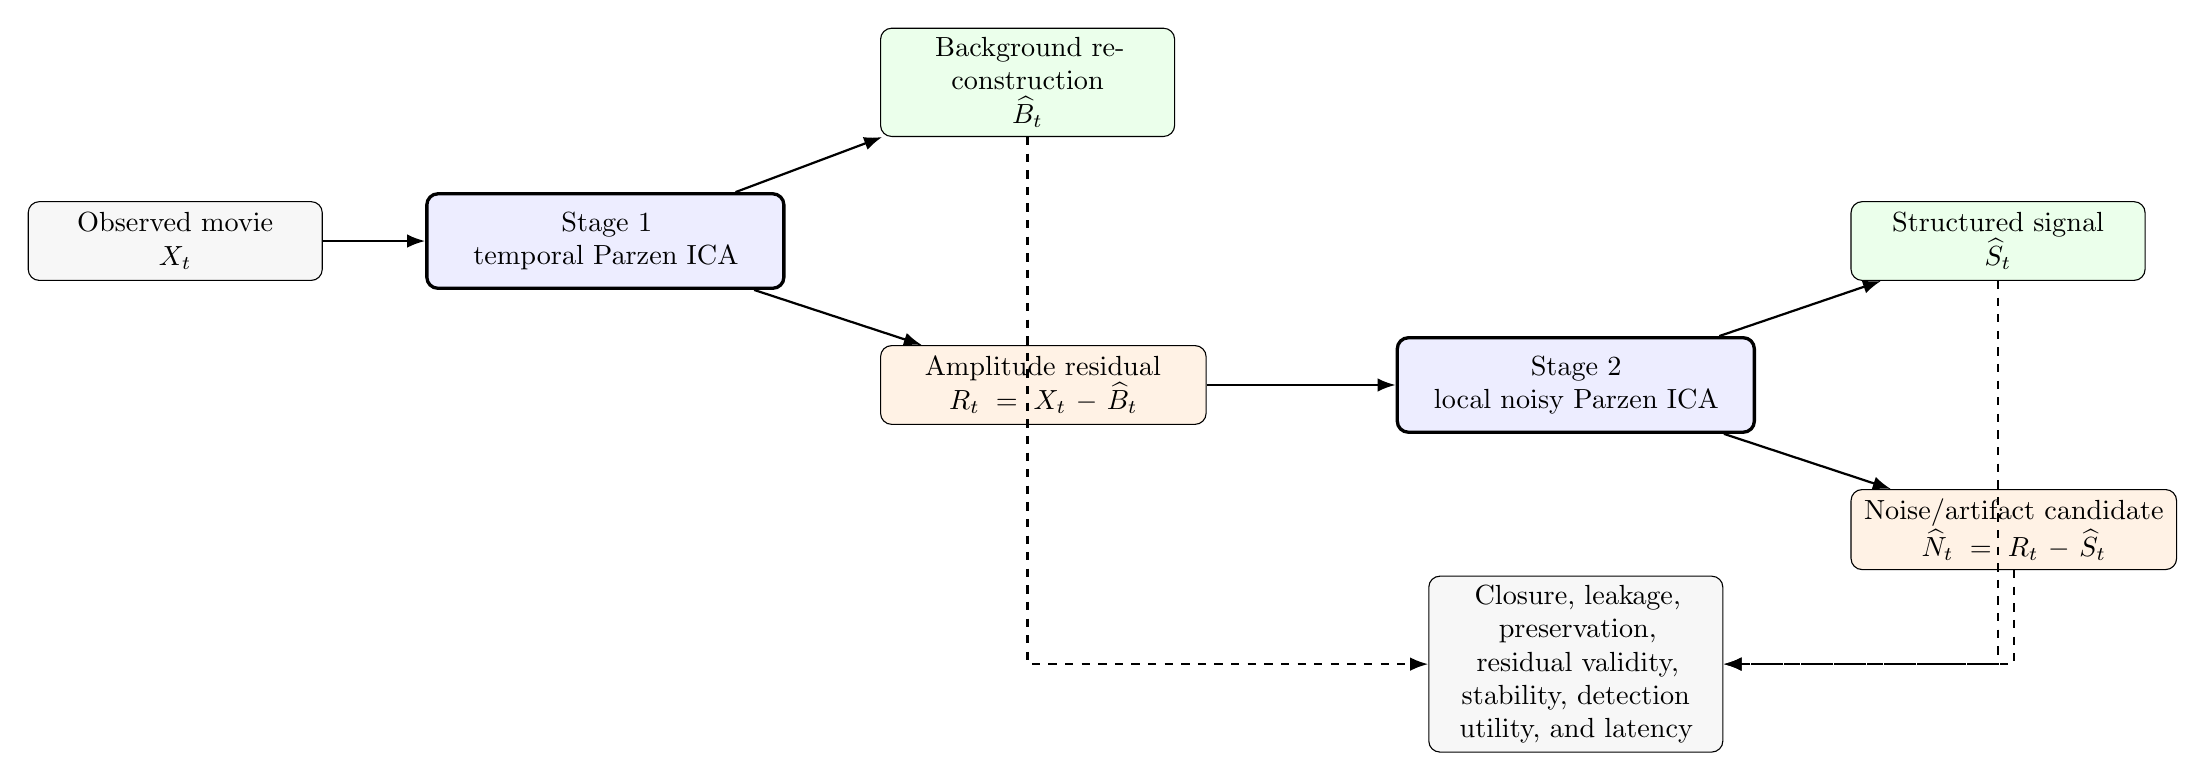
\begin{tikzpicture}[
  node distance=8mm and 13mm,
  box/.style={draw, rounded corners, align=center, minimum height=10mm,
              text width=35mm, fill=black!3},
  stage/.style={draw, rounded corners, align=center, minimum height=12mm,
                text width=43mm, fill=blue!7, very thick},
  output/.style={draw, rounded corners, align=center, minimum height=10mm,
                 text width=35mm, fill=green!8},
  residual/.style={draw, rounded corners, align=center, minimum height=10mm,
                   text width=39mm, fill=orange!10},
  arrow/.style={-{Latex[length=2.3mm]}, thick}
]
\node[box] (raw) {Observed movie\\$X_t$};
\node[stage, right=of raw] (s1) {Stage 1\\temporal Parzen ICA};
\node[output, above right=7mm and 12mm of s1] (bg) {Background reconstruction\\$\widehat B_t$};
\node[residual, below right=7mm and 12mm of s1] (r) {Amplitude residual\\$R_t=X_t-\widehat B_t$};
\node[stage, right=24mm of r] (s2) {Stage 2\\local noisy Parzen ICA};
\node[output, above right=7mm and 12mm of s2] (sig) {Structured signal\\$\widehat S_t$};
\node[residual, below right=7mm and 12mm of s2] (noise) {Noise/artifact candidate\\$\widehat N_t=R_t-\widehat S_t$};
\node[box, below=18mm of s2] (diag) {Closure, leakage, preservation, residual validity,\\stability, detection utility, and latency};

\draw[arrow] (raw) -- (s1);
\draw[arrow] (s1) -- (bg);
\draw[arrow] (s1) -- (r);
\draw[arrow] (r) -- (s2);
\draw[arrow] (s2) -- (sig);
\draw[arrow] (s2) -- (noise);
\draw[arrow, dashed] (bg) |- (diag);
\draw[arrow, dashed] (sig) |- (diag);
\draw[arrow, dashed] (noise) |- (diag);
\end{tikzpicture}}
\caption{Proposed reversible hierarchy. Stage~1 uses temporal mixtures to
estimate background but passes an amplitude-preserving residual rather than a
derivative component. Stage~2 estimates structured sources under an additive
noise model. The final residual is validated rather than presumed to be noise.}
\label{fig:hierarchy}
\end{figure}

\section{What the existing NeuRev results imply}

The proposal follows from three repository-level findings.

\subsection{Pairwise ICA became a temporal derivative}

For adjacent observations at pixel \(p\),
\begin{equation}
\bm x_t(p)=
\begin{bmatrix}
I_{t-1}(p)\\ I_t(p)
\end{bmatrix}.
\end{equation}
Persistent structure lies near \([1,1]^\top\); the orthogonal background-null
direction is \([-1,1]\). The fitted InfoMax and CS-Parzen directions in the
initial NeuRev experiment were nearly collinear with subtraction. This is a
useful empirical result, but it means the non-background output is approximately
\begin{equation}
\Delta I_t = \Delta S_t + \Delta N_t + \Delta O_t,
\end{equation}
not a clean neural signal.

For independent frame noise with variance \(\sigma^2\),
\begin{equation}
\Var(N_t-N_{t-1})=2\sigma^2.
\label{eq:diff-noise}
\end{equation}
Temporal subtraction cancels common structure while amplifying high-frequency
measurement noise.

\subsection{Amplitude survived where differencing failed}

The completed latent-dynamics benchmark found that the offline smoother
amplitude improved known-label recovery, whereas raw/latent differences,
positive dynamic drive, and filter innovation underperformed. The representation
benchmark similarly found a small provisional gain from low-rank amplitude PCA,
while high-rank ICA became unstable. Table~\ref{tab:anchors} records the current
anchors that the proposed method must reproduce before comparison.

\begin{table}[H]
\centering
\caption{Current NeuRev anchors. These are prior experiment results, not results
of the proposed hierarchy. Candidate counts are not ordinary false positives
because labels are sparse.}
\label{tab:anchors}
\begin{tabularx}{\textwidth}{>{\raggedright\arraybackslash}Xrrrr}
\toprule
Lane & Known matches & Labels & Candidates & Comment \\
\midrule
Raw Direct, latent-dynamics contract & 49 & 79 & 232 & Frozen amplitude anchor \\
Causal AR(1) filter amplitude & 53 & 79 & 312 & Causal; 2/4 burst wins \\
Offline RTS smoother amplitude & 55 & 79 & 320 & Noncausal; 4/4 burst wins \\
Raw Direct, fixed 58/burst budget & 52 & 79 & 232 & Representation anchor \\
Amplitude PCA rank 8, fixed budget & 54 & 79 & 232 & Provisional two-match gain \\
\bottomrule
\end{tabularx}
\end{table}

\begin{figure}[H]
\centering
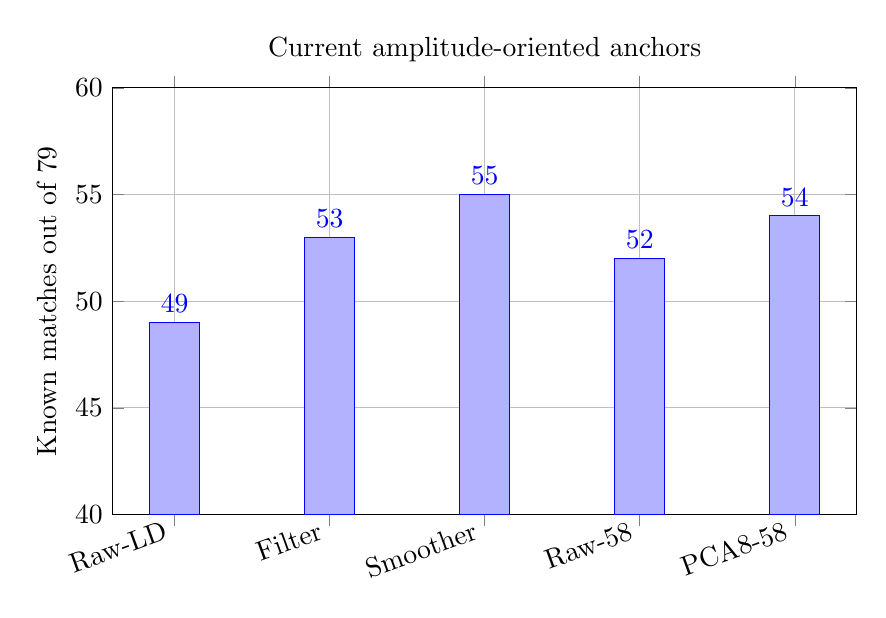
\begin{tikzpicture}
\begin{axis}[
  width=0.91\textwidth,
  height=7cm,
  ybar,
  ymin=40, ymax=60,
  ylabel={Known matches out of 79},
  symbolic x coords={Raw-LD,Filter,Smoother,Raw-58,PCA8-58},
  xtick=data,
  x tick label style={rotate=20,anchor=east},
  nodes near coords,
  bar width=18pt,
  grid=major,
  title={Current amplitude-oriented anchors}
]
\addplot coordinates {(Raw-LD,49) (Filter,53) (Smoother,55) (Raw-58,52) (PCA8-58,54)};
\end{axis}
\end{tikzpicture}
\caption{The strongest current evidence favors denoised or low-rank amplitude,
not derivative-only evidence. Different evaluation policies are displayed
separately and must not be numerically conflated.}
\label{fig:anchors}
\end{figure}

\section{Stage 1: temporal Parzen ICA}

\subsection{Temporal embeddings and identifiability boundary}

The mandatory embedding is
\begin{equation}
\bm x^{(2)}_t(p)=
[I_{t-1}(p),I_t(p)]^\top.
\end{equation}
A gated extension uses
\begin{equation}
\bm x^{(3)}_t(p)=
[I_{t-2}(p),I_{t-1}(p),I_t(p)]^\top.
\end{equation}
Reference temporal directions are shown in Fig.~\ref{fig:temporalgeometry}.

\begin{figure}[H]
\centering
\resizebox{0.92\textwidth}{!}{%
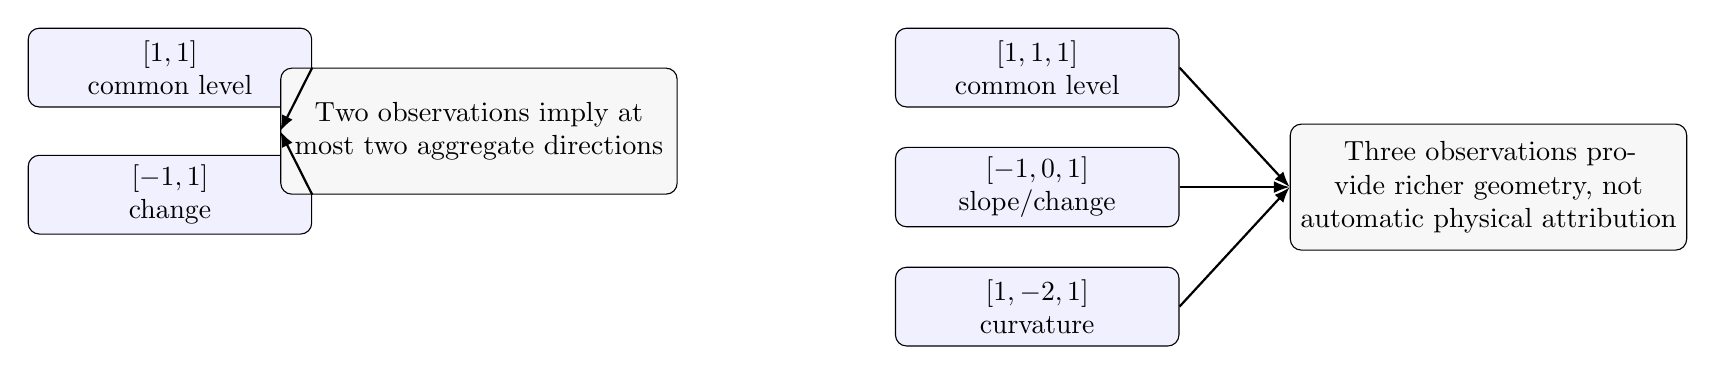
\begin{tikzpicture}[
  vec/.style={draw,rounded corners,align=center,minimum width=36mm,
              minimum height=10mm,fill=blue!6},
  note/.style={draw,rounded corners,align=center,text width=48mm,
               minimum height=16mm,fill=black!3},
  arrow/.style={-{Latex[length=2mm]},thick}
]
\node[vec] (c2) {$[1,1]$\\common level};
\node[vec, below=6mm of c2] (d2) {$[-1,1]$\\change};
\node[note, right=14mm of $(c2)!0.5!(d2)$] (n2) {Two observations imply at most two aggregate directions};
\draw[arrow] (c2.east) -- (n2.west);
\draw[arrow] (d2.east) -- (n2.west);

\node[vec, right=74mm of c2] (c3) {$[1,1,1]$\\common level};
\node[vec, below=5mm of c3] (s3) {$[-1,0,1]$\\slope/change};
\node[vec, below=5mm of s3] (q3) {$[1,-2,1]$\\curvature};
\node[note, right=14mm of s3] (n3) {Three observations provide richer geometry, not automatic physical attribution};
\draw[arrow] (c3.east) -- (n3.west);
\draw[arrow] (s3.east) -- (n3.west);
\draw[arrow] (q3.east) -- (n3.west);
\end{tikzpicture}}
\caption{Reference temporal directions. ICA may rotate and scale these
directions, but the embedding dimension bounds the number of aggregate
components.}
\label{fig:temporalgeometry}
\end{figure}

The embedding does not make background, neural state, and noise jointly
identifiable. Stage~1 is therefore an aggregate background-reconstruction model,
not a claim of full physical source separation.

\subsection{Parzen independence criterion}

After robust centering and whitening,
\begin{equation}
\bm z_i=Q(\bm x_i-\bm\mu),
\end{equation}
we fit an orthogonal demixer \(W_1\) so that
\begin{equation}
\bm y_i=W_1\bm z_i.
\end{equation}
The batch reference uses a bounded Parzen information-theoretic independence
criterion. Quadratic R\'enyi and Cauchy--Schwarz functionals estimated with
Parzen windows provide nonparametric contrasts, but their bandwidth controls
smoothness, variance, and optimization geometry~\cite{erdogmus2004deconv,principe2010}.

A stochastic lane follows the stochastic information-gradient concept of
Erdogmus, Hild, and Principe~\cite{erdogmus2003sig}. Its purpose is bounded
online adaptation, not a new source of identifiability. The implementation must
retain a finite dictionary or replay buffer, symmetric decorrelation, gradient
and update limits, deterministic seeds, and fallback to the preceding valid
demixer.

\subsection{Background assignment}

The component with derivative \emph{mean} closest to zero is not necessarily
background; zero-mean noise also satisfies that condition. For component
\(y_j(t)\), use robust normalized derivative energies
\begin{equation}
E_{1,j}=
\frac{\operatorname{median}_t(\Delta y_j(t))^2}
{\Var(y_j)+\epsilon},
\qquad
E_{2,j}=
\frac{\operatorname{median}_t(\Delta^2 y_j(t))^2}
{\Var(y_j)+\epsilon}.
\end{equation}
A soft background score combines these with global-intensity correlation,
low-spatial-frequency mass, spatial breadth, motion-edge correlation, and
window-to-window continuity. The assignment may be unresolved. A low score
margin triggers a declared fallback rather than an arbitrary background label.

This caution is essential because slowly rising or persistent calcium activity
can also have small adjacent derivatives. If
\begin{equation}
s_t=\gamma s_{t-1}+u_t,
\end{equation}
then
\begin{equation}
\Delta s_t=(\gamma-1)s_{t-1}+u_t.
\end{equation}
When \(\gamma\) is close to one, real neural state can appear nearly static over
one frame.

\subsection{Background reconstruction and amplitude residual}

Let \(A_1=Q^{-1}W_1^{-1}\) denote the map from ICA coordinates to observation
coordinates, with the centering term handled explicitly. For selected
background-component set \(\mathcal B\), reconstruct the current-frame
coordinate:
\begin{equation}
\Bhat_t(p)=
\bm e_{\mathrm{current}}^\top
A_{1,\mathcal B}\bm y_{i,\mathcal B} + b_{\mathrm{current}}.
\end{equation}
Then pass
\begin{equation}
R_t(p)=I_t(p)-\Bhat_t(p)
\label{eq:stage1-residual}
\end{equation}
to Stage~2. The method retains \(I_t\), \(\Bhat_t\), and \(R_t\); it never
passes only the derivative-like ICA output.

\section{Stage 2: local noisy Parzen ICA}

\subsection{Noisy generative model}

For one overlapping image patch,
\begin{equation}
\bm r_t=A_2\bm s_t+\bm n_t,
\label{eq:noisy-ica}
\end{equation}
where \(\bm s_t\) contains a bounded number of structured latent sources and
\(\bm n_t\) is additive observation noise plus model error. This differs from
ordinary ICA, which effectively treats all retained variation as a noiseless
linear mixture. Explicit noisy ICA has been shown to improve source estimation
when noise covariance and source densities are modeled~\cite{cordes2007}.

Noise is not represented as an ordinary ICA component. Multiple Gaussian noise
sources are rotationally ambiguous, and artifacts may be structured. Stage~2
instead estimates structured sources and leaves an explicitly tested residual.

\subsection{Quiet noise covariance and signal subspace}

From held-out quiet Stage-1 residuals, estimate \(\widehat\Sigma_n\). The
mandatory reference is robust diagonal covariance; a diagonal-plus-low-rank
model is a gated extension. For residual covariance \(\widehat\Sigma_r\), form
\begin{equation}
\widehat\Sigma_s=
\operatorname{PSD}\!\left(
\widehat\Sigma_r-\widehat\Sigma_n
\right).
\label{eq:noise-corrected-cov}
\end{equation}
Only stable positive modes enter the ICA subspace. A zero-rank patch is a valid
outcome. Ordinary PCA whitening remains an ablation because it does not subtract
estimated noise energy.

Spectral covariance matching and joint diagonalization methods such as SMICA
provide a relevant noisy-source baseline~\cite{ablin2020smica}. Local PMD,
CNMF/CNMF-E, and OASIS provide complementary functional-imaging controls that
explicitly exploit low-rank, spatial, or calcium-dynamics structure
\cite{buchanan2018,pnevmatikakis2016,zhou2018,friedrich2017}.

\subsection{Noise-convolved Parzen source density}

For scalar latent source \(s_j\), define a Gaussian Parzen prior
\begin{equation}
\widehat p_{s_j}(s)=
\frac{1}{M}\sum_{m=1}^{M}
\N(s;c_{jm},h_j^2).
\label{eq:source-parzen}
\end{equation}
If projected additive noise is
\begin{equation}
\eta_j\sim\N(0,\sigma_j^2),
\end{equation}
then the observed output \(y_j=s_j+\eta_j\) has density
\begin{equation}
\widehat p_{y_j}(y)=
\frac{1}{M}\sum_{m=1}^{M}
\N\!\left(y;c_{jm},h_j^2+\sigma_j^2\right).
\label{eq:noisy-parzen}
\end{equation}
This analytic convolution is the core noise-aware modification. The Parzen
bandwidth \(h_j\) and projected physical noise variance \(\sigma_j^2\) remain
separate recorded parameters.

The posterior kernel responsibility is
\begin{equation}
\alpha_{jm}(y)=
\frac{\N(y;c_{jm},h_j^2+\sigma_j^2)}
{\sum_{\ell=1}^{M}\N(y;c_{j\ell},h_j^2+\sigma_j^2)}.
\end{equation}
Within kernel \(m\), Gaussian conditioning gives
\begin{equation}
\mu_{jm}(y)=
\frac{\sigma_j^2c_{jm}+h_j^2y}{h_j^2+\sigma_j^2},
\qquad
v_{jm}=
\frac{h_j^2\sigma_j^2}{h_j^2+\sigma_j^2}.
\end{equation}
Therefore
\begin{equation}
\widehat s_j(y)=
\sum_m\alpha_{jm}(y)\mu_{jm}(y),
\label{eq:posterior-mean}
\end{equation}
with mixture posterior variance
\begin{equation}
\widehat v_j(y)=
\sum_m\alpha_{jm}(y)
\left[v_{jm}+\mu_{jm}(y)^2\right]
-\widehat s_j(y)^2.
\label{eq:posterior-var}
\end{equation}
The method thus emits a denoised source amplitude and uncertainty, not merely an
independent noisy output.

\subsection{Noisy stochastic score and update}

Let
\begin{equation}
\overline c_j(y)=\sum_m\alpha_{jm}(y)c_{jm}.
\end{equation}
The negative score of the noisy Parzen mixture is
\begin{equation}
\psi_j(y)=
-\frac{\partial}{\partial y}\log\widehat p_{y_j}(y)
=
\frac{y-\overline c_j(y)}{h_j^2+\sigma_j^2}.
\label{eq:noisy-score}
\end{equation}
A reference natural-gradient update is
\begin{equation}
W_2\leftarrow
W_2+\rho
\left[I-\bm\psi(\bm y_t)\bm y_t^\top\right]W_2,
\label{eq:natural-update}
\end{equation}
followed by symmetric decorrelation. The update is a falsifiable implementation
choice, not a guarantee of global convergence. The stochastic-information-
gradient literature supports bounded online Parzen updates
\cite{erdogmus2003sig,yang2007}, but the explicit noise convolution in
Eqs.~\eqref{eq:noisy-parzen}--\eqref{eq:noisy-score} is what makes this stage
noise aware.

Dictionary centers should initially be frozen. A later EM-like refresh may use
posterior clean-source means rather than raw noisy outputs. Append-only
dictionaries are prohibited.

\subsection{Source acceptance, reconstruction, and residual}

A component is accepted as structured signal only when it has reproducible
spatial/temporal structure, adequate posterior SNR, bounded uncertainty, low
motion-edge correlation, and synthetic source-recovery value. Accepted posterior
means reconstruct
\begin{equation}
\Shat_t=A_2\widehat{\bm s}_t,
\end{equation}
then
\begin{equation}
\Nhat_t=R_t-\Shat_t.
\label{eq:noise-candidate}
\end{equation}
Overlapping patches use a declared overlap-add window and emit disagreement maps.
A coherent annulus, event-locked trace, broad drift, or moving edge in \(\Nhat_t\)
is evidence of model mismatch.

\section{Reversible refinement and cascade risk}

A hard hierarchy can erase signal. If Stage~1 estimates
\begin{equation}
\Bhat=B+\delta S,
\end{equation}
then Stage~2 receives only \((1-\delta)S+N\). No second-stage method can infer the
removed fraction from the residual alone. Therefore every run preserves the raw
movie, Stage-1 component contributions, background, and amplitude residual.

A gated one-pass refinement may update
\begin{equation}
\Bhat^{\mathrm{refined}}
\leftarrow
\arg\min_B\norm{X-B-\Shat}_F^2+R_B(B)
\end{equation}
inside a strict trust region around the initial background, followed by one
Stage-2 refit. This ablation is allowed only after the non-refined reference
passes attribution gates.

\section{Metrics for the overarching goal}

\subsection{Numerical accounting}

Define
\begin{equation}
E^{\mathrm{closure}}=X-\Bhat-\Shat-\Nhat.
\end{equation}
Report median, p95, p99, maximum, and nonfinite count by frame and patch. Closure
is necessary but not sufficient: an arbitrary split can close perfectly.

\subsection{Attribution leakage}

For true channels \(C_i\in\{B,S,N\}\) and estimates
\(\widehat C_j\in\{\Bhat,\Shat,\Nhat\}\), report
\begin{equation}
L^{\mathrm{corr}}_{ij}=
\frac{\langle C_i,\widehat C_j\rangle_F^2}
{(\norm{C_i}_F^2+\epsilon)(\norm{\widehat C_j}_F^2+\epsilon)}.
\label{eq:leakage}
\end{equation}
Also report energy-attribution regressions so each true channel's energy is
accounted for across estimated channels and unexplained error. Success requires a
stable diagonally dominant matrix, especially low signal leakage into background
and noise.

\subsection{Neural preservation}

At synthetic/injected and known events, report peak-amplitude ratio, temporal-area
ratio, onset/peak/duration/decay error, centroid error, footprint IoU, annular
overlap, event energy in background, and event-locked residual energy. Detection
recall cannot substitute for these preservation metrics.

\subsection{Residual validity}

The final residual is tested through temporal ACF, spatial ACF, PSD ratio to
held-out quiet noise, intensity-conditioned variance calibration, event locking,
motion-edge correlation, and tail/outlier maps. A non-Gaussian residual is not
automatically invalid; it indicates that the declared Gaussian model may be
insufficient.

\subsection{Optimization and scientific stability}

Report objectives, gradients, demixer changes, orthogonality error, dictionary
occupancy, bandwidth/noise sensitivity, matched component correlations, subspace
angles, assignment margins, patch disagreement, candidate Jaccard, and failure
rates across seeds, temporal blocks, and nearby hyperparameters.

\subsection{Downstream detection}

Compare single features under both quiet calibration and a fixed 58-candidate
per-burst budget. Report per-burst known recall, candidates, localization,
shared misses, and candidate overlap. Unmatched candidates remain unknown. Any
later fusion initializes exactly at Raw Direct with auxiliary weights at zero.

\subsection{Latency}

Separate frozen per-frame inference from slow adaptation. Report p50, p95, p99,
maximum, memory, and throughput for both stages, posterior inference,
overlap-add, and detection. At 50~Hz, p95 frozen/causal software latency must be
below 20~ms before real-time eligibility.

\section{Experiments}

\subsection{Fully synthetic temporal and noisy-source tests}

Stage~1 tests static background, drift, photobleaching, slow neural ramps,
plateaus, gain change, impulses, and translated edges. Stage~2 tests varied
source distributions, source dependence, SNR, colored/heteroscedastic noise,
Poisson--Gaussian approximations, outliers, rank mismatch, covariance mismatch,
and source-distribution drift.

\subsection{Semi-synthetic movies}

Inject known disks, annuli, membrane arcs, overlapping cells, border cells, and
diffuse zones into real quiet Spon backgrounds. Cross bounded event kinetics,
SNR, footprint size, local brightness, gain drift, translation, and saturation
proximity. Preserve separate true \(B,S,N,O\) channels.

\subsection{Real-data sequence}

After synthetic gates:
\begin{enumerate}[leftmargin=*]
\item tiny read-only smoke;
\item frozen Stage-1 diagnostic;
\item Stage-2 local diagnostic on a bounded review interval;
\item denoising/preservation report;
\item single-feature detection comparison;
\item optional bounded fusion;
\item latency profile;
\item full Spon run only after explicit selection.
\end{enumerate}

\section{Required visual results}

All visual comparisons use fixed scales and machine-readable source data.
Placeholders below are replaced automatically when the report artifacts are
placed under `figures/`.

\begin{figure}[H]
\centering
\resultfigure{figures/fixed_scale_channel_montage.png}{0.96\linewidth}{7.0cm}
\caption{Required six-channel montage: raw observation, reconstructed background,
Stage-1 amplitude residual, Stage-2 structured signal, noise/artifact candidate,
and closure residual.}
\label{fig:montage}
\end{figure}

\begin{figure}[H]
\centering
\begin{subfigure}[t]{0.49\linewidth}
\centering
\resultfigure{figures/leakage_matrix.png}{0.98\linewidth}{5.2cm}
\caption{Median attribution leakage matrix.}
\end{subfigure}
\hfill
\begin{subfigure}[t]{0.49\linewidth}
\centering
\resultfigure{figures/closure_by_frame.png}{0.98\linewidth}{5.2cm}
\caption{Numerical closure by frame.}
\end{subfigure}
\caption{The principal decomposition-accounting figures.}
\label{fig:accounting}
\end{figure}

\begin{figure}[H]
\centering
\begin{subfigure}[t]{0.49\linewidth}
\centering
\resultfigure{figures/stage1_diagnostics.png}{0.98\linewidth}{5.2cm}
\caption{Stage-1 component reconstruction and assignment.}
\end{subfigure}
\hfill
\begin{subfigure}[t]{0.49\linewidth}
\centering
\resultfigure{figures/stage2_diagnostics.png}{0.98\linewidth}{5.2cm}
\caption{Stage-2 maps, traces, posterior means, and uncertainty.}
\end{subfigure}
\caption{Component-level interpretation.}
\label{fig:components}
\end{figure}

\begin{figure}[H]
\centering
\resultfigure{figures/parzen_posteriors.png}{0.90\linewidth}{5.5cm}
\caption{Latent Parzen densities, noise-convolved observed densities,
responsibilities, posterior source estimates, and uncertainty across
representative noise levels.}
\label{fig:parzen-post}
\end{figure}

\begin{figure}[H]
\centering
\begin{subfigure}[t]{0.49\linewidth}
\centering
\resultfigure{figures/signal_preservation.png}{0.98\linewidth}{5.2cm}
\caption{Amplitude, area, timing, and footprint preservation.}
\end{subfigure}
\hfill
\begin{subfigure}[t]{0.49\linewidth}
\centering
\resultfigure{figures/residual_validity.png}{0.98\linewidth}{5.2cm}
\caption{Temporal/spatial ACF, PSD, calibration, and event locking.}
\end{subfigure}
\caption{Biological preservation and residual validity.}
\label{fig:preservation-residual}
\end{figure}

\begin{figure}[H]
\centering
\begin{subfigure}[t]{0.49\linewidth}
\centering
\resultfigure{figures/recall_tradeoff.png}{0.98\linewidth}{5.2cm}
\caption{Known recall versus candidate burden.}
\end{subfigure}
\hfill
\begin{subfigure}[t]{0.49\linewidth}
\centering
\resultfigure{figures/latency_breakdown.png}{0.98\linewidth}{5.2cm}
\caption{Frozen inference and slow adaptation latency.}
\end{subfigure}
\caption{Downstream utility and operational feasibility.}
\label{fig:utility-latency}
\end{figure}

\section{Advancement gates}

\begin{table}[H]
\centering
\small
\caption{Stage-gated decision contract. Exact thresholds are preregistered in the
experiment manifest and report.}
\label{tab:gates}
\begin{tabularx}{\textwidth}{>{\bfseries}p{0.08\textwidth}X}
\toprule
Gate & Requirement \\
\midrule
G0 & Exact contracts, finite deterministic outputs, collision-safe artifacts,
Raw Direct reproduction, and focused tests. \\
G1 & Stage-1 background reconstruction improves relevant baselines, median neural
leakage to background is below the declared bound, event amplitude/area are
preserved, and ambiguous assignments are not forced. \\
G2 & Noisy Parzen posterior source recovery improves ordinary Parzen ICA in the
predefined noisy regimes, uncertainty is calibrated under matched cases, and
accepted components are stable. \\
G3 & End-to-end closure passes and the median background--signal--noise leakage
matrix is diagonally dominant across seeds and perturbations. \\
G4 & Real neural/injected events preserve amplitude, temporal area, timing, and
footprint, with no material event-locked residual. \\
G5 & At fixed candidate budget, known recall improves consistently, or candidate
burden falls materially without known-label loss. Upstream failed gates cannot be
overridden by detection gain. \\
G6 & Frozen causal p95 software latency is below the frame deadline, with stable
component continuity and bounded slow updates. \\
\bottomrule
\end{tabularx}
\end{table}

\section{Failure modes and interpretation}

\subsection{Signal absorbed into Stage-1 background}

This is the dominant cascade risk. It is detected through injected event leakage,
known-event energy in \(\Bhat\), low assignment margin, and Stage-1 residual loss.
The response is unresolved fallback or bounded refinement, not a more aggressive
Stage-2 method.

\subsection{Background leakage accepted as structured signal}

Broad drift or motion structure may be non-Gaussian and therefore attractive to
ICA. Spatial breadth, low-frequency mass, motion-edge correlation, quiet
calibration, and residual attribution are required to reject it.

\subsection{Noise-covariance mismatch}

If intensity-dependent or correlated noise is approximated as diagonal Gaussian,
posterior shrinkage and rank selection can be wrong. Intensity-variance,
spatial-ACF, and quiet-holdout diagnostics determine whether a richer noise model
is justified.

\subsection{Parzen degeneracy}

Small bandwidths produce rough objectives and sparse responsibilities; large
bandwidths wash out higher-order structure. Dictionary collapse, stale centers,
responsibility saturation, and gradient starvation/explosion must be reported.
The physical noise variance may not be hidden inside the selected bandwidth.

\subsection{Dependent neural sources}

Synchronized neurons violate strict source independence. In such regimes, the
structured source \emph{subspace} may be more identifiable than individual
components. Report subspace recovery and do not force one-neuron-per-component
claims.

\subsection{Visually clean but scientifically wrong decomposition}

Low-rank background can absorb neural events, and a powerful source model can
reconstruct artifacts. Therefore visual quality, entropy gain, reconstruction
loss, and detection recall are all secondary to attribution leakage, signal
preservation, residual validity, and stability.

\section{Relation to alternative methods}

CNMF and CNMF-E jointly model spatial footprints, temporal activity, background,
and noise using functional-imaging constraints~\cite{pnevmatikakis2016,zhou2018}.
PMD separates localized low-dimensional structure from approximately
unstructured noise before downstream demixing~\cite{buchanan2018}. OASIS infers
sparse calcium drives after a trace has been defined~\cite{friedrich2017}. These
are necessary baselines and potential extensions.

The proposed hierarchy is most compelling when it demonstrates that
information-theoretic nonparametric source models add measurable value beyond
those structured controls, particularly under non-Gaussian or multimodal source
distributions, while retaining explicit uncertainty and real-time-capable frozen
inference.

\section{Conclusion}

The proposed method is summarized by
\begin{equation}
\boxed{
\begin{gathered}
\text{temporal Parzen ICA for background reconstruction}\\[-1mm]
\Downarrow\\[-1mm]
\text{local noisy Parzen ICA for structured-signal estimation}
\end{gathered}}
\end{equation}
with the unexplained residual validated rather than presumed to be noise. The
claim is not that the hierarchy guarantees perfect separation. The claim to be
tested is that explicit channels, noise-aware posterior inference, reversible
intermediate artifacts, and falsification-oriented metrics can produce a more
stable and scientifically useful background--signal--noise attribution than
ordinary pairwise ICA, ordinary noisy residual filtering, or unconstrained
high-rank representations.

\bibliographystyle{IEEEtran}
\bibliography{references}

\end{document}
